\documentclass[a4paper]{article}

\usepackage[english]{babel}
\usepackage[utf8x]{inputenc}
\usepackage{amsmath}
\usepackage{graphicx}
\usepackage[colorinlistoftodos]{todonotes}
\usepackage{color}
\usepackage{hyperref}
\usepackage{fullpage}

\title{Open Information Systems\\Assignement part 2 }
\author{Matteo Marra, Antoine Carpentier, Titouan Christophe, Bruno Rocha Pereira}

\begin{document}
\maketitle

\todo{read over this fcking shit}
\todo{RATING owns a RECORD (not the other way around) => RECORD::rating is optional}

\section{Introduction}

Our application will help users to share and rate their favorite locations and tracks for exercises of all sorts. Users will interact in three ways : 

\begin{enumerate}
    \item Record and share tracks (where they run, bike...)
    \item Tag those tracks with specific keywords for other users to discover them
    \item Record and share spots where they exercise along tracks
\end{enumerate}

The following sections develop each of the three points above, then we discuss
the database organization.

\section{Tracks}

When a user wants to record its use of a new or existing track, our application will track its movement and record the starting and ending time. The user will have to specify which activity type he is doing (e.g. running, biking...) and optionally rate their record (with a grade and a review). Our application will be able to determine if the user is using a new track, in which case, the application will record it automatically.

The length of the track will be computed only once when the user saves and stored in the database for performance issues. It will indeed never change and should be stored even if it redundant.

The tracks will be displayed on a map in our application. This will allow users to clearly see the path the track follows.

\section{Tags}

Users will be able to tag tracks with keywords and search tracks based on these keywords. Each track will have none, one or several tags attached to it and one tag will be able to relate to several tracks. That way, users will find tracks related to their interests and methods of exercising.

\section{Exercise spots}

Along the tracks, users will be able to specify spots where they exercise (a specific location where they practice a sport or a part of a track that they like). They will be allowed to rate these spots with a grade up to 5 stars and an optional review to permit other users to discover these spots.
When a user views a specific track, the spots will be displayed with their ratings.

\section{Description of the database}

\subsection{Implementation}
We use PostgreSQL\footnote{\url{http://www.postgresql.org/}} with the PostGis\footnote{\url{http://postgis.net/}} geographic extension as our database engine.

\begin{figure}[h]
    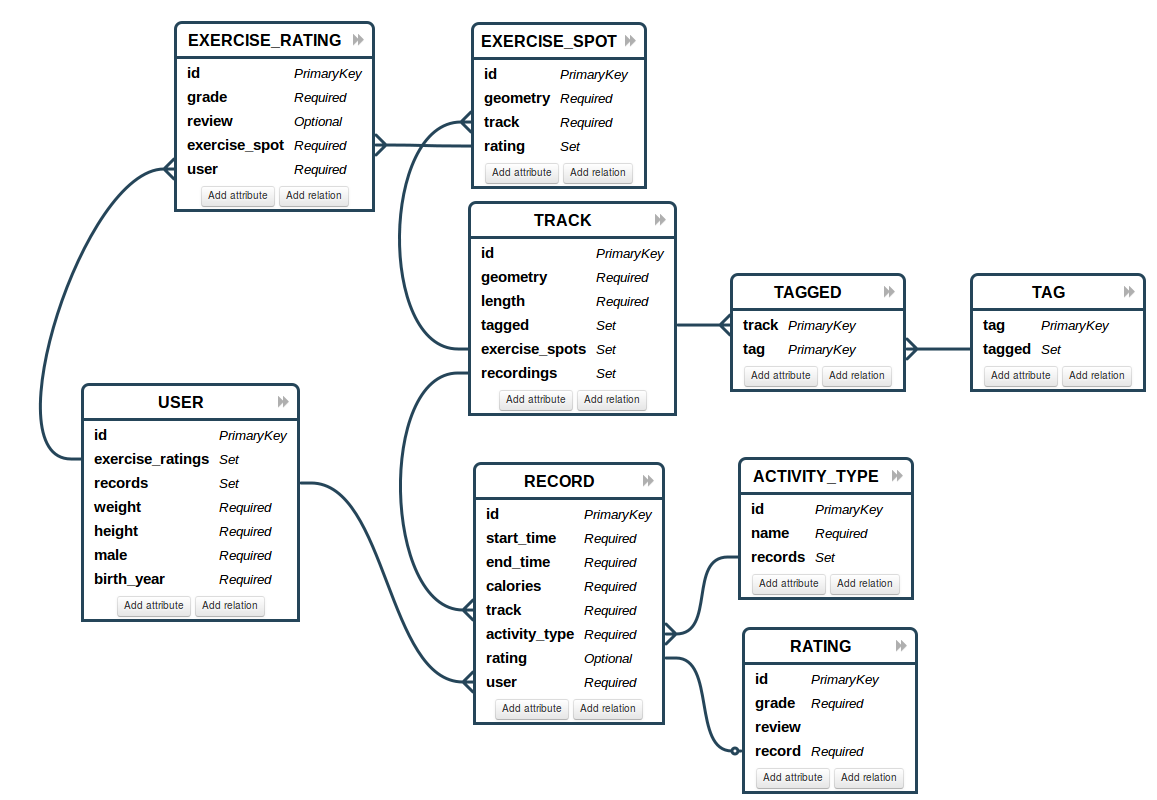
\includegraphics[width=\textwidth]{er-diagram.png}
    \caption{Entity Relationship diagram}
\end{figure}


\subsection{User}
A user contributes to the information system by creating an account and providing
some information about its body. These informations are used to approximate the
number of calories spent by users on different tracks.

\paragraph{id} For now, we suppose that a user only has an unique identifier (integer)
\paragraph{weight} Its weight, in kg (integer)
\paragraph{height} Its height, in cm (integer)
\paragraph{male} Indicate whether the user is female (\texttt{false}) or male (\texttt{true})

Using "male" instead of gender allows ut to restrain the values to being boolean (instead of for example integers that would have too many possible values).


\subsection{Track}
The central model of our database is a \textbf{Track}, which consists of:

\paragraph{id} Its identifier (integer)
\paragraph{geometry} A geographic linestring of gps records (latitude, longitude, elevation)
\paragraph{length} Its length in meters (float)

Using gps recorders, a user can create geographic traces of their activities on
their smartphones and upload them to our information system. For example a GPX\footnote{\url{http://www.topografix.com/gpx.asp}}
file importer might be implemented.


\subsection{Tag}
Users can then add tags to the tracks, which are simply strings to quickly find
tracks according to the user mood.


\subsection{Exercice Spot}
All along these tracks, users could also insert informations about the exercises
point they find. An exercice point is a large notion including special variations
of a track, exercising devices, or even sport halls and public infrastructures.

\paragraph{id} Its identifier (integer)
\paragraph{geometry} A collection of geographic features (points, lines, etc...)
\paragraph{track} The track this exercise spot belongs to


\subsection{Record}
When a user goes for a run on a track included in the databse, he can record his
performance and provide an optional rating.

\paragraph{id} Its identifier (integer)
\paragraph{start\_time, end\_time} The beginning and the end of the activity (datetime)
\paragraph{calories} The number of calories spent  (float). We could approximate this number with the user's personal data, or rely on external services like smartphone and health oriented devices if possible.
\paragraph{track} The track used
\paragraph{user} The user who made the activity
\paragraph{activity\_type} The kind of activity (see below)


\subsection{Activity Type}
As users might bike, run, walk, and have other exercise activities on the tracks,
our database also lists different activity types.

\paragraph{id} Its identifier (integer)
\paragraph{name} The activity type name (string)


\subsection{Ratings}
User can optionally provide ratings for their records, and exercises spots.

\paragraph{id} Its identifier (integer)
\paragraph{grade} A general appreciation from 0 to 5 stars(integer)
\paragraph{review} An optional description of the review

\end{document}
